% This is samplepaper.tex, a sample chapter demonstrating the
% LLNCS macro package for Springer Computer Science proceedings;
% Version 2.21 of 2022/01/12
%
\documentclass[runningheads]{llncs}
%
\usepackage[T1]{fontenc}
% T1 fonts will be used to generate the final print and online PDFs,
% so please use T1 fonts in your manuscript whenever possible.
% Other font encondings may result in incorrect characters.
%
\usepackage{graphicx}
% Used for displaying a sample figure. If possible, figure files should
% be included in EPS format.
%
% If you use the hyperref package, please uncomment the following two lines
% to display URLs in blue roman font according to Springer's eBook style:
%\usepackage{color}
%\renewcommand\UrlFont{\color{blue}\rmfamily}
%
\usepackage[ngerman]{babel}
\usepackage{wrapfig}
\begin{document}
%
\title{Gruppe 3: Catchphrase?}
%
%\titlerunning{Abbreviated paper title}
% If the paper title is too long for the running head, you can set
% an abbreviated paper title here
%
\author{...\inst{1}\and
...\inst{1}\and
...\inst{1}\and
...\inst{1}}
%
\authorrunning{F. Author et al.}
% First names are abbreviated in the running head.
% If there are more than two authors, 'et al.' is used.
%
\institute{FernUniversität in Hagen, Universitätsstraße 47, 58097 Hagen, Deutschland
\email{\{...\}@studium.fernuni-hagen.de}\\
\url{https://www.fernuni-hagen.de}}
%
\maketitle              % typeset the header of the contribution
%
%
\section{Einleitung}
TODO Gruppenbeschreibung
\section{Kommunikation und Kommunikationsmittel}
TODO Gruppentreffen, Github

\section{Technische Rahmenbedingungen und Softwarebasisarchitektur}
TODO Java, Bdi, 2 Agentensysteme, UML

\section{Gruppenbeitrag Heinz Stadler}
Nach einer ausführlichen Einarbeitung in die Thematik der Multiagentensysteme, erfolgte die Analyse der Ergebnisse des 15. Multi-Agent Programming Contest \cite{Ahlbrecht2021}. Diese ergab, dass neben der Entscheidungsfindung der Agenten, der Aufbau einer konsistenten und umfangreichen Wissensbasis (vgl. \cite[S. 29]{Ahlbrecht2021}) sowie die effiziente Problemfindung (vgl. \cite[S. 17]{Ahlbrecht2021}), eine wesentliche Schwierigkeit der Aufgabe bilden. \\
Als Folge dessen entschied sich der Autor mit dem Aufbau der Wissensverwaltung (siehe \ref{wissensverwaltung}) zu beginnen. Diese umfasst eine Datenstruktur zur Speicherung der von der Simulation übermittelten Informationen, sowie eine Lösung zum Aufbau einer globalen Karte des Simulationsgebiets. Nach Fertigstellung der Karte und deren funktionalen Verifikation, wurde parallel an der Konzeptionierung des Agentensystem V1 (siehe \ref{agentV1}) sowie der Implementierung einer intelligenten Wegführung (siehe \ref{wegfindung}) gearbeitet. Um die Ergebnisse der Wegführung und das Entscheidungsverhalten der Agenten effektiv verifizieren zu können, folgte die Erstellung eines graphischen Analysewerkzeugs (siehe \ref{verifikation}) das im weiten Entwicklungsverlauf stetig weiterentwickelt wurde und sich als sehr hilfreich bei der Fehlerfindung zeigte.
 
\subsection{Agent V1 - Architektur}\label{agentV1}
\begin{wrapfigure}{r}{0.56\linewidth}
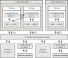
\includegraphics{./Referenzen/Architekturdiagramm.pdf}
\caption{Architekturdiagramm Agent V1}
\label{g3:architecture}
\end{wrapfigure}
Das Agentensystem V1 wurde vom Autor konzipiert, in der Gruppe abgestimmt und schließlich selbstständig implementiert. Es erweitert das BDI-Konzept \cite{Bratman1987} um zusätzliche Daten-, Berechnungs- und Entscheidungsebenen, die in Abbildung \ref{g3:architecture} illustriert sind. \\
Das System kombiniert den Aufbau eines BDI-Agenten (vgl. \cite[S. 58]{Weiss2000}) mit einer bidirektionalen vertikalen Schichtarchitektur \cite[S. 61-62]{Weiss2000}, auf die in Abschnitt
\ref{absichtsfindung} näher eingegangen wird.

Jeder Agent wurde mit einer Vorgesetzteninstanz, die eine zusätzliche Entscheidungsebene bildet, kombiniert und in einem Thread parallelisiert. Werden Agenten zu einer Gruppe zusammengeführt, bleibt eine Vorgesetzeninstanz aktiv. Die sonstigen Instanzen der Gruppe werden passiv und übernehmen im Weiteren nur noch die Weiterleitung von Nachrichten an die aktive Entität.

Die Kommunikation zwischen Instanzen in verschiedenen Threads erfolgt über Nachrichten, die in einer threadsicheren Warteschlange zwischengespeichert werden. Die Verständigung des Agenten mit seinem direkten Vorgesetzten wird mittels Methodenaufrufen realisiert.

Agentengruppen aktualisieren eine gemeinsame Karte mit im Simulationsverlauf erhaltenen Umgebungsinformationen. Diese und Module zur Wegführung werden von einem zentralem threadsicheren Navigationsmodul, das als Einzelstück ausgeführt wurde, verwaltet. 


\subsection{Wissensverwaltung}\label{wissensverwaltung}
Jeder Agent hat Zugriff auf eine individuelle Wissensbasis (Beliefs), die von der Simulation bereitgestellte Informationen auswertet und speichert. \\
Die enthaltenen Umgebungsdaten, beschränken sich auf das aktuelle Sichtfeld des Agenten. Es ist weder die Größe des Simulationsgebiets, noch die absolute Position des Agenten in diesem bekannt. 
Um aus den partiellen Umgebungsinformationen eine globale Sicht zu erhalten, werden diese an das Navigationsmodul weitergeleitet und in einer chronologisch fortgeschriebenen Karte zusammengeführt.

Beim Simulationsstart erhält jeder Agent, eine Karte mit festgelegter Initialgröße (Abb. \ref{Karte} Punkt 1), die beim Erkunden der Umgebung erweitert wird (Abb. \ref{Karte} Punkt 2). Treffen sich zwei Agenten aus unterschiedlichen Gruppen, wird dies vom Navigationsmodul erkannt und an die aktiven Vorgesetzten beiden Gruppen gemeldet. Stimmen beide Vorgesetzte einer Vereinigung zu, werden deren Karten überlagert und schließlich zusammengeführt (Abb. \ref{Karte} Punkt 3). Die zusammengeführte Karte ermöglicht nun im weiteren Simulationsverlauf die aktuelle Position aller Agenten einer Gruppe untereinander zu bestimmen. Aus dieser Information kann nun durch jeweils zwei Agenten, die sich in entgegengesetzte Richtungen bewegen und sich durch das kontinuierliche Simulationsgebiet zwangsläufig wieder treffen, die Kartengröße ermittelt werden. Ist dies erfolgt, wird die Karte beschnitten, wobei die Informationen abgeschnittener Bereiche auf der gegenüberliegenden Seite eingefügt werden und somit nicht verloren gehen (Abb. \ref{Karte} Punkt 4).
\begin{figure}[h]
\includegraphics{./Referenzen/Kartenmerge.pdf}
\caption{Erweiterung und Zusammenführung einzelner Karten}
\label{Karte}
\end{figure}

\subsection{Wegfindung}\label{wegfindung}
Die 
Pathfinding, 2 Stufiges System

\subsection{Ziel- und Absichtsfindung}\label{absichtsfindung}
Desires, verticale Schichtarchitektur

\begin{wrapfigure}{r}{0.56\linewidth}
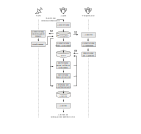
\includegraphics{./Referenzen/Entscheidungsfindung.pdf}
\caption{Architekturdiagramm Agent V1}
\label{g3:architecture}
\end{wrapfigure}

\subsection{Verifikation und Problemfindung}\label{verifikation}
Tests / Debugger

\subsection{Rekapitulation}
Zahlen, sonstiges Server Bug, Turnier gehalten, Github erstellt

\subsection{...}

\section{Gruppenbeitrag Melinda Betz}

\section{Gruppenbeitrag Phil Heger}

\section{Gruppenbeitrag Björn Wladasch}

\section{Turniere}
\subsubsection{Turnier 2}
\subsubsection{Turnier 3}
\subsubsection{Turnier 4}
\subsubsection{Turnier 5}
\subsubsection{Turnier 6}

\section{Rekapitulation und Ausblick}
Vor- und Nachteile der Entscheidung von zwei Architekturen
Was sollte noch verbessert werden
Wie sind wir zufrieden


%
% ---- Bibliography ----
%
% BibTeX users should specify bibliography style 'splncs04'.
% References will then be sorted and formatted in the correct style.
%
% \bibliographystyle{splncs04}
% \bibliography{mybibliography}
%
\begin{thebibliography}{8}
	\bibitem{Ahlbrecht2021}
	Ahlbrecht, T., Dix, J., Fiekas. N. und T. Krausburg: The Multi-Agent Programming Contest 2021, Springer, Heidelberg, 2021
	\bibitem{Hart1968}
	Hart, P. E., Nilsson, N. J. und Raphael, B.: A Formal Basis for the Heuristic Determination of Minimum Cost Paths, in IEEE Transactions on Systems Science and Cybernetics, 4. Auflage, Nummer 2, Seiten 100-107, Juli 1968
	\bibitem{Weiss2000}
	Weiss, G.: Multiagent Systems, 2. Auflage, The MIT Press, Cambridge, 2000
	\bibitem{EISMASSim}
	github.com/agentcontest/massim\_2022, agentcontest/massim\_2022, \\ https://github.com/agentcontest/massim\_2022/blob/main/docs/eismassim.md, EISMASSim Documentation, 21.08.2022
	\bibitem{Bratman1987}
	Bratman, M.: Intention, plans, and practical reason, Harvard University Press, Cambridge, 1987
\end{thebibliography}
\end{document}
